\documentclass{article}
\usepackage{spconf,amsmath,graphicx,tabularx,color,url,subfigure}

../../reproducible/tex/definitions.tex
\global\long\def\neil#1{{\color{red} \textbf{#1}}}

\title{Ranking of Gene Regulators through Differential Equations and Gaussian Processes}

\name{Antti Honkela$^1$, Marta Milo$^2$, Matthew Holley$^3$, Magnus
  Rattray$^4$, and Neil D. Lawrence$^4$\thanks{A.H. was supported by
    Postdoctoral Researcher's Project No 121179 of the Academy of
    Finland.  M.R. and N.D.L acknowledge support from EPSRC Grant No
    EP/F005687/1 "Gaussian Processes for Systems Identification with
    Applications in Systems Biology".  This work was supported in part
    by the IST Programme of the European Community, under the PASCAL2
    Network of Excellence, IST-2007-216886. This publication only
    reflects the authors' views.}}
\address{$^1$ Department of Information and Computer
    Science,\\ Aalto University School of Science and Technology,
    Helsinki, Finland\\
  $^2$ School of Medicine and Biomedical Science,
    NIHR Cardiovascular Biomedical Research Unit,\\
    Sheffield Teaching Hospitals NHS Trust, Sheffield, UK \\
  $^3$ Department of Biomedical Science, University of Sheffield, UK \\
  $^4$ School of Computer Science, University of
    Manchester, UK}

\begin{document}

\maketitle

\begin{abstract}
  Gene regulation is controlled by transcription factor proteins which
  themselves are encoded as genes. This gives a network of interacting
  genes which  control the functioning of  a cell. With  the advent of
  genome   wide   expression  measurements   the   targets  of   given
  transcription  factor have  been sought  through techniques  such as
  clustering. In this paper we  consider the harder problem of finding
  a  gene's regulator instead  of its  targets.  We  use a  model-based
  differential  equation  approach combined  with  a Gaussian  process
  prior distribution for unobserved continuous-time regulator expression
  profile.  Candidate regulators can then be ranked according to model
  likelihood.  This idea,
  that  we refer  to as  ranked  regulator prediction  (RRP), is  then
  applied   to  finding   the  regulators   of  Gata3,   an  important
  developmental transcription  factor, in the development  of ear hair
  cells.
\end{abstract}

\sloppy

\section{INTRODUCTION}

Gene regulation is at the heart of how cells operate. In transcription
genes  which are  encoded in  the  DNA are  transcribed to  messenger
RNA.  The  quantity of  RNA  transcribed  can  be measured  genome-wide
through the  well established approach of gene  expression arrays. The
mechanisms  by   which  transcription  is  controlled   are  of  great
importance for medicine and biology.  Expression of a gene is switched
on  and off by  transcription factors  (TF), proteins
which bind to the DNA. The  TF proteins are produced by translation of
TF mRNA  that  is  also
transcribed from  the genome.  This implies that  at the heart  of the
cell there is a network of TFs controlling the regulation of target genes and
governing  the function  of  the  cell. Unpicking  this  network is  a
central  aim of  computational systems  biology. High  throughput gene
expression experiments allow the expression  level of many genes to be
assessed  simultaneously.  A typical  analysis  involves  a series  of
experiments  (perhaps a  time  series) for  which  gene expression  is
obtained.  Then   cluster  analysis  can   be  performed  and   it  is
hypothesized that genes that are  members of the same cluster (and are
therefore   probably  well   correlated   to  one   another)  may   be
coregulated.  Confirmation  experiments  may then  involve  ``knocking
out'' the  regulating gene and looking  for a resulting  change in the
gene expression of the hypothesized targets.

\subsection{Model-Based Ranking}

Recently a  model-based  approach to ranking  of targets  was proposed
that extends  this idea to  include an explicit  differential equation
model  of   gene  expression  \cite{Barenco:ranked06}. This  allows
ranking of coregulated genes even when the expression profiles are not
strongly  correlated due to different decay  rates. The  basic form  of the
model is as follows
\begin{equation}
  \diff{m_i(t)}{t} = b_i + s_i p(t) - d_i m_i(t)
\end{equation}
where the mRNA concentration of the $i$th gene, $m_i(t)$ is assumed to
be  regulated by  the TF  of interest,  $p(t)$, through  a sensitivity
parameter $s_i$.  The decay  rate of  the mRNA is  given by  $d_i$ and
$b_i$  is a  basal rate  of transcription.  Solution of  this equation
gives
\begin{equation}
  m_i(t) = a_i e^{-d_it} + \frac{b_i}{d_i} + s_i
  e^{-d_it}\int_0^tp(u)e^{d_i u}\mathrm{d} u \label{eq:linearOperator}
\end{equation}
and the initial condition is given by $m_i(0)=a_i + \frac{b_i}{d_i}$. 

If coregulated targets have similar decay rates, they will be strongly
correlated, but  if decay  rates differ then  targets can  become more
weakly correlated.  The  idea behind the model-based  approach is to
consider that  coregulated targets should conform  to the differential
equation. Thus  we see  a TF activity,  $p(t)$, that  explains targets
simultaneously through  a range of different decay  rates.  Clearly we
are also making further assumptions  here: for example we are assuming
TFs  do not act  in tandem  and  that the  response to  the TF  does not
saturate. Other regulatory mechanisms, such as chromatin remodelling
and non-coding RNAs are also ignored as they are typically unobserved.
However,  the model is richer than  the standard genome-wide
analysis   techniques  of  seeking   correlation  or   clustering  the
data. This model-based approach to gene regulation was also considered
in  \cite{Gao:latent08}. They  used Gaussian  process priors  over the
unobserved TF activity  to create a fully probabilistic  model for the
coregulated genes.
%  Likelihoods can then  be used to rank these models
%and determined which genes are likely to be coregulated.

Also in \cite{Gao:latent08} this framework was extend by introducing a
simple model  of translation.  Let us represent the  mRNA governing the
transcription factor by $m_0(t)$. Let us assume that this is translated
to  $p(t)$ through a  process that  can be  modelled by  the following
differential equation
\begin{equation}
  \diff{p(t)}{t} = m_0(t) - \delta p(t).
\end{equation}
Once again this  is a significant simplification. It  assumes that the
TF  protein is  produced from  only one  mRNA and  ignores potentially
important post translational  modifications such as phosphorylation or
ubiquitination.

Given  observations  from the  potential  target  mRNA, $m_i(t)$,  and
observations  from the  governing TF's  mRNA a  joint  Gaussian process
likelihood can be constructed  and maximized with respect to $\delta$,
$a_i$,  $b_i$,  $s_i$  and  $d_i$.  For  a  given  TF  this
likelihood can be measured for all potential target genes and they can
then  be ranked  as  putative  targets.  This  idea  was exploited  by
\cite{Honkela:modelbased10}  who validated  their  results using  ChIP
data  and  were  able to  show  that  model-based approaches  can  do
considerably better than simple correlation-based approaches.

In this paper we want to turn this idea on its head. Instead of asking
what  the targets are  of a  particular TF  we wish  to know  what the
regulator of a particular gene is. In other words we are interested in
ranked regulator prediction instead  of ranked target prediction.
The proposed approach is otherwise fairly similar with respect to the
methods to that in~\cite{Honkela:modelbased10}.

The ranked regulator prediction (RRP)
problem will generally  be harder than target prediction  as there are
likely to be many targets of a particular TF, but only few regulators.
However, we  can restrict  ourselves to known  TFs when  searching for
regulators  and this reduces  the number  of genes  we have  to search
through from thousands to hundreds.  RRP
has the  potential to provide biologists  with a new  tool for probing
their regulatory networks.

In the  remainder of  this paper we  will review the  Gaussian process
approach to  modelling transcriptional regulation  and demonstrate our
ideas  on a  real world  biological problem.  Despite  the simplifying
assumptions we make, we show very promising results.

\section{Gaussian Process Modelling}

A  Gaussian  process (GP)  is  a  probabilistic  prior over  functions
\cite{Rasmussen:book06}.  A GP  provides a  nonparametric  approach to
modelling data. The  basic idea is that observations  of a function of
interest,   $p(t)$,   given  by   $\mathbf{p}   =  \left[p_1,   \dots,
  p_T\right]^\top$,   where    $p_i=p(t_i)$   are   jointly   Gaussian
distributed,
\begin{equation}
  \mathbf{p} \sim \mathcal{N}(\mathbf{0}, \mathbf{K}).
\end{equation}
where the elements of the  covariance matrix are given by a covariance
function. This may  be any function that leads  to a positive definite
matrix, but a common choice is the Gaussian covariance,
\begin{equation}
  k(t_i,   t_j)   =  \frac{\sigma^2}{\sqrt{2\pi   \ell^2}}\exp\left(-\frac{(t_i
      -t_j)^2}{2\ell^2}\right).
\end{equation}
Whilst we usually  think of Gaussians as being  densities over finite
length vectors, the process perspective  allows us to think of them as
distributions over infinite length vectors. The important idea is that
the  other  possible things  that  could  be  happening are  all  been
marginalized, and we only  deal with the observations $\mathbf{p}$. If
we need to  query a new observation time, $p_*$,  we express the joint
distribution over the augmented variable set as
\begin{equation}
  \left[\begin{matrix}
      \mathbf{p}\\
      \mathbf{p}_*
    \end{matrix}\right]
  \sim \mathcal{N}\left(\mathbf{0}, \left[\begin{matrix}
        \mathbf{K} & \mathbf{K}_{:,*}\\
        \mathbf{K}_{*,:} & \mathbf{K}_{*,*}
      \end{matrix}
    \right]\right),
\end{equation}
where $\mathbf{K}_{:,*}$  is the covariance  function computed between
the training  times, $\mathbf{t}$, and the  test times, $\mathbf{t}_*$
and $\mathbf{K}_{*,*}$ is the covariance function computed between the
test times.

Simple  manipulation of  this joint  Gaussian  density, $p(\mathbf{p},
\mathbf{p_*}|\mathbf{t},  \mathbf{t}_*)$,  allows  us to  compute  the
conditional density of the test data given the training data,
\begin{equation}
  p(\mathbf{p}_* | \mathbf{p}, \mathbf{t}, \mathbf{t}_*) = \mathcal{N}\left(\mathbf{p}_*|\boldsymbol{\mu}, \boldsymbol{\Sigma}\right)
\end{equation}
where
\begin{equation}
  \boldsymbol{\mu} = \mathbf{K}_{*,:}\mathbf{K}^{-1}\mathbf{p}
\end{equation}
and 
\begin{equation}
  \boldsymbol{\Sigma} = \mathbf{K}_{*,*} - \mathbf{K}_{*,:}\mathbf{K}^{-1}\mathbf{K}_{:,*}.
\end{equation}

The simple  translation/transcription model  we described in  the last
section gives  a deterministic  relationship between the  TF activity,
$p(t)$  and the gene  expression levels,  $m_0(t)$ and  $m_i(t)$. This
deterministic relationship can be encoded within a GP by
noting  that it  is  given  by a  \emph{linear  operator}. The  linear
operator  in question  is  the  convolution of  the  function with  an
exponential  (see  \refeq{eq:linearOperator}).   A  convolution  of  a
GP  with  a  deterministic function  leads  to  another
GP: this results from two properties, a GP
multiplied by a deterministic function  is also a GP and
the integral  of a  GP is  also a GP. The
other effect  of \refeq{eq:linearOperator} is to introduce  a new mean
function through  the addition  of $\frac{b_i}{d_i}$ and  $a_i e^{-d_i
  t}$.            Details            are           given            in
\cite{Lawrence:transcriptionalGP06,Gao:latent08,Honkela:modelbased10}
but  the main  result is  that the  cross covariances  between  the TF
concentration and the mRNA concentrations can be computed:
\begin{align*}
  k_{m_0, m_i}(t, t^\prime) = & s_i e^{-d_i t^\prime} \int_0^{t^\prime}
  e^{(d_i - \delta) u} \int_0^u e^{\delta v} k(t, v)\, \mathrm{d}v\, \mathrm{d}u \\
  = & \frac{s_i \sigma^2e^{-(d_i+\delta) t^\prime}}{\sqrt{8}(\delta - d_i)} \\
  &\times\bigg( e^{\left(\frac{d_i \ell}{2}\right)^2 + d_i t +
    \delta t^\prime }
  \big[\erf(d_i \ell / 2 + t/\ell) \\
  &\quad - \erf(d_i \ell / 2 + (t-t^\prime)/\ell)\big] \\
  &-e^{\left(\frac{\delta \ell}{2}\right)^2 + \delta t + d_i
    t^\prime} \big[\erf(\delta \ell / 2 + t/\ell) \\
  &\quad- \erf(\delta \ell / 2 +
  (t-t^\prime)/\ell)\big] \bigg).
\end{align*}
where $k_{m_0,m_i}(t, t^\prime)$ gives the covariance between the mRNA
of the TF and the mRNA associated with the $i$th gene at times $t$ and
$t^\prime$.  The covariance function between a target gene and itself is given by
\begin{align*}
  k_{m_j, m_k}(t, t^\prime) = &s_j s_k e^{-d_j t - d_k t^\prime}\\
  &\times\int_0^t e^{(d_j - \delta) u}
  \int_0^{t^\prime} e^{(d_k - \delta) u'} \\
  &\times
  \int_0^u e^{\delta v} \int_0^{u'} e^{\delta v'} k(v, v') \, \mathrm{d}v'\, \mathrm{d}v\, \mathrm{d}u'\, \mathrm{d}u \\
  = &\frac{\sigma^2 s_j s_k}{\sqrt{8}} \bigg(
  h_{jk}(t, t^\prime, \delta) + h_{kj}(t^\prime, t, \delta) \\
  &- h_{jk}(t, t^\prime, d_j) - h_{kj}(t^\prime, t, d_k)
  \bigg)
\end{align*}
where
\begin{align*}
  h_{jk}(t, t^\prime,& d_x) =  e^{\left(\frac{d_x \ell}{2}\right)^2}
  \frac{e^{-d_x t - d_k t^\prime}}{(d_x + \delta) (d_j - \delta)} \\
  &\times\Bigg\{
   %\frac{(d_k + \delta)\exp((d_k-\delta) t^\prime) - 2\delta}{(d_k^2-\delta^2)}
  \left(\frac{e^{(d_k-\delta) t^\prime} - 1}{d_k-\delta} +
    \frac{1}{d_k + d_x} \right)\\
  &\times \left[\erf\left(\frac{d_x \ell}{2} - \frac{t}{\ell}\right) - \erf\left(\frac{d_x \ell}{2}\right)\right]
  \\
  &+ \frac{e^{(d_k+d_x)t^\prime}}{d_k+d_x}\\
  &\times\left[\erf\left(\frac{d_x \ell}{2} + \frac{t^\prime}{\ell})
  - \erf(\frac{d_x \ell}{2} - \frac{(t-t^\prime)}{\ell}\right)\right]
  \bigg\}.
\end{align*}
If we  observe a Gaussian noise corrupted  version of the
true   profiles,   where   the    noise   covariance   is   given   by
$\boldsymbol{\Sigma}$ (which  typically would  be constrained to  be a
diagonal  or spherical  matrix) this  suggests  a model  for the  gene
expression which is jointly Gaussian and has the form
\begin{equation}
  \left[\begin{matrix}
      \mathbf{m}_0\\
      \mathbf{m}_i
    \end{matrix}\right]
  \sim \mathcal{N}\left(\left[\begin{matrix}\mathbf{0}\\\boldsymbol{\mu}\end{matrix}\right], \left[\begin{matrix}
        \mathbf{K}_{0,0} & \mathbf{K}_{0,i}\\
        \mathbf{K}_{i,0} & \mathbf{K}_{i,i}
      \end{matrix}
    \right] + \boldsymbol{\Sigma}\right),
\end{equation}
where the $m$, $n$th element of the matrix $\mathbf{K}_{0,0}$ is given
by   $k(t_m,t_n)$,    for   $\mathbf{K}_{0,i}$   it    is   given   by
$k_{m_0,m_i}(t_m,  t_n)$ and for  $\mathbf{K}_{i, i}$  it is  given by
$k_{m_i, m_i}(t_m,  t_n)$. Here $t_m$ and $t_n$  are observation times
from the time  series data. The mean values are  derived from the mean
functions.   So  we  have  the  $j$th  element  of  the  mean  vector,
$\mu_j=\frac{b_i}{d_i}  +  a_ie^{-d_it_j}$.   Since  these  covariance
functions and  mean functions are  all dependent on the  parameters of
the differential equations, $\sigma$, $\delta$, $a_i$, $s_i$ and $d_i$
we can fit these parameters  by gradient-based maximization of the log
likelihood of a given pairing  of regulator and target gene (using the
scaled conjugate gradient  algorithm of \cite{Moller:scg93}). This can
be done in turn for each  potential regulator of the target gene.  The
regulator genes  can the be  ranked according to which  model achieves
the highest likelihood.



\section{Experiments}

%\neil{We need more specifics on the quality of these results. Currently we are being very wishy washy.}

Careful experimental validation of the proposed method is very
difficult as practically the only systems where the ground truth is
known as synthetic.  These are, however, unrepresentative as the
results are highly dependent on the details of the experimental setup
and the degree of presence of confounding factors.  With these
considerations in mind, we demonstrate the method in preliminary
analysis of candidate regulators of Gata3 gene in  mouse.  More
careful biological validation of the results is needed for full
evaluation, but that is beyond the scope of the current work.

Our example gene Gata3 is itself   a transcription factor with several
important  functions~\cite{Chou2010}.  For example  it is  critical in
the development of hair cells in  the inner ear.  Mice and humans with
just  one of  the usual  two  copies of  the Gata3  gene disabled  are
deaf~\cite{Esch2000}.  Gata3 has many  roles causing its regulation to
be  very  complex.  The  details  of  this  regulation  are  currently
relatively poorly understood~\cite{Burch2005}.

We considered a gene expression data set consisting of two time series
from     a    cell     line     model    of     mouse    inner     ear
development~\cite{Helyer:model07}.   The  cell  line is  derived  from
sensory epithelial cells from the  ventral part of the otic vesicle at
E10.5  and cultured  in  serum-free  media. It  was  produced from  12
hybridisations to  the Affymetrix GeneChip® Mg\_U74Av2.  The cells for
both  time series  are  cultured for  a  period of  14  days to  mimic
development of  the otic  vesicle and sampled  in $6$ time  points, at
$0$,  $1$, $2$,  $4$,  $7$  and $14$  days  after differentiation  was
stimulated (through  temperature change).  In  one of the  time series
the  cells  are untreated  while  in the  other  they  are exposed  to
retinoic acid, which focuses the differentiation toward one of several
possible cell types.  The retinoic  acid treatment does not affect the
expression profile  of Gata3 so  we used these  two time series  as if
they  were  two   repeated  experiments.   This  should  automatically
suppress genes with significant  differential expression under the two
different  conditions.  The  expression data  was processed  using the
mmgMOS       algorithm        from       the       \emph{puma}       R
package~\cite{Liu:tractable04,Pearson:puma09}  from Bioconductor.  The
inferred posterior  expression levels from mmgMOS were  used to obtain
individual   noise  variances  for   each  observation   as  described
in~\cite{Honkela:modelbased10}  using  the  \emph{tigre}  Bioconductor
package. %~\cite{Honkela:tigrepackage10}.

We first extracted a set of  mouse TFs and probable TFs from the TFCat
database~\cite{Fulton2009}.  This yielded a list of 511 genes.  Out of
these,  365  were  mappable  on  the  array  used  in  the  expression
measurements.  These  genes were represented by  493 independent probe
sets on the array.

For some genes the signal from the expression measurements is too weak
for reasonable modelling: they can  be described perfectly with a flat
profile.  Such genes may nevertheless  fit the model well, but this is
non-informative because  they would fit equally well  as regulators of
any  other  gene.   These  genes  were filtered  by  z-scores  of  the
expression      data     using      the      cut-off     $1.8$      as
in~\cite{Honkela:modelbased10}.  This filtering left 268 active probes
sets.

Next, we fitted the GP models independently using each of these 268 TF
gene  probes as  the input  and Gata3  as the  output.  This  was also
performed in R/Bioconductor using the \emph{tigre} package. We considered the top ranked 50 genes in this list. 

Pathways like Wnt signaling, TGF-beta signaling and PDGF signaling are
involved  in  pattering of  sensory  patch,  development and  neuronal
differentiation  as  well  as  modulation  of  cell  fate.  All  these
processes  are expected to  be highly  represented in  this particular
cell line, which is derived  from a murine sensory epithelial cells at
embryonic age E9.5~\cite{Milo2009}.

%The top ranked 10 potential regulators of Gata3 from our model were
%(in order): Prrx2, \textbf{Tle3}, Ctbp2, Smarcd2, \textbf{Six1}, Runx2,
%Mtf2, Six4, Arntl and \textbf{Tbx6}.
The top ranked 10 potential regulators of Gata3 from our model were
(in order): Prrx2, Tle3, Ctbp2, Smarcd2, Six1, Runx2,
Mtf2, Six4, Arntl and Tbx6.

To truly validate our  predictions biological assays are required, but
we can get  a preliminary insight in the validity of  the ranking by a
protein  analysis using  the  classification system  known as  PANTHER
(Protein     ANalysis     THrough     Evolutionary     Relationships),
\url{http://www.pantherdb.org/}.   PANTHER uses hidden  Markov models,
knowledge of  existing protein families and  sub-families to classify the
role of a given protein.  PANTHER then uses a binomial statistics tool
to  compare  classifications  of  multiple  clusters  of  lists  to  a
reference  list. This allows  it to  statistically determine  over- or
under- representation of the defined categories. Each list is compared
to   the  reference  list.   To  determine   statistical  significance
$p$-values  are   also  calculated  using   the   Benferroni-corrected
test. The  $p$-values are the  probabilities that the number  of genes
observed  in a  category  occurred  by chance,  as  determined by  the
reference list. A small $p$-value indicates that the category selected
is significant  and potentially interesting.   We used as  a reference
list  the NCBI:Mus  Musculus genome.  The  selected list  of genes  is
compared  against  this  baseline  and  for each  PANTHER  pathway  an
estimated  number   of  genes  are  calculated   with  their  relative
$p$-values. Those  having $p$-values that were significant  at the 5\%
level  are shown  in  Table \ref{tab:pathways}.  They  are all  highly
relevant to the development of the mammalian inner ear.

\begin{table}[tb]
  \caption{Enriched pathways among 50 top-ranking candidate regulators.}
  % \neil{How were these selected? Are they the only ones? How highly ranked were they?}}
  \label{tab:pathways}
 \centering
  \begin{tabularx}{\columnwidth}{Xl}
    Pathway & $p$-value \\
    \hline
    Wnt signaling pathway &	$4.10\times 10^{-6}$ \\
    TGF-beta signaling pathway & $2.22\times 10^{-2}$ \\
    Inflammation mediated by chemokine and cytokine signaling pathway & $4.18\times 10^{-2}$ \\
    Interleukin signaling pathway & $4.81\times 10^{-1}$\\
    % Wnt signaling pathway	408	9	.68	+	$4.10\times 10^{-6$}
    % TGF-beta signaling pathway	154	4	.26	+	$2.22\times 10^{-2}$
    % Inflammation mediated by chemokine and cytokine signaling pathway	337	5	.56	+	$4.18\times 10^{-2}$
    % Interleukin signaling pathway	169	3	.28	+	$4.81\times 10^{-1}$
  \end{tabularx}
\end{table}

%\neil{What is this bit? [Tables of most relavant pathways can be extracted from the file.]}

Looking at the 50 highest ranking TFs as candidate regulators of Gata3
we find  that the list is  highly enriched for genes  belonging to the
Wnt signaling  pathway.  From the top  10 ranked TFs we  note that the
list includes  Six1. Sine  oculis homeobox (SIX)  protein family  is a
group of  evolutionarily conserved  transcription factors that  play a
key role in development. Particularly,  Six1 is known to be related to
a  defective  otic development  known  as brachio-oto-renal  syndrome.
This  syndrome   is  autosomal  dominant   disorder  characterized  by
syndromic  association  of  branchial  cysts or  fistulae  along  with
external, middle and inner ear malformations and renal anomalies. Mice
without Six1 show sever malformation  of the middle and inner ear with
cochleae completely  lacking of hair  cells \cite{Bosman2009}. Further
Six1 promotes differentiation and regulation of cell fate in the inner
ear~\cite{Fritzsch2007,Bosman2009}.  Gata3  is  a  key player  in  the
development  of the inner  ear, it  promotes cell  differentiation and
patterning in the inner ear  and regulates the development of the otic
neurons.  In addition,  only one  copy of  functional Gata3  in human,
causes HDR syndrome (hypoparathyroidism, deafness, renal dysplasia), a
syndrome  that  presents similar  phenotype  to the  brachio-oto-renal
syndrome.   This   evidence   reinforces   the   possible   functional
relationship between  the two  genes and therefore  makes Six1  a very
interesting  candidate  for  further  investigation.  Note  also  that
another TF that is known to act together with Six1 is also ranked very
high in the in the list: Six4. The Wnt signaling related gene Tbx6 and
the notch  signaling related  gene Tle3 are  also of interest  in this
context,  since modulation  of Notch  signaling and  Wnt  signaling is
crucial for normal patterning during embryogenesis. The inner ear is a
very  complex  organ in  which  patterning  play  a crucial  role  for
ensuring  the mechanotransduction  properties of  the organ.  Both the
T-box  and Groucho/Tle  gene families  are highly  conserved  and many
studies  in  fish  and  flies  have revealed  their  crucial  role  in
development of  sensory organ. The  connection of Gata3 with  both Wnt
and     Notch    signaling    is     known    in     the    literature
\cite{Rivolta2002,Kelly2009}, Tbx6  and Tle3 are  potentially two very
interesting modulators  of the effect of  Gata3 on both  these two key
signalling pathways. Based on the known protein annotation, ontologies
and published literature, the model has identified several interesting
candidates  as  Gata3 regulators.  However,  more detailed  functional
assays  are required  to properly  assess the  biological  property of
these relationships  in this particular biological system,  as well as
general effect that these targets  can have on the modulation of Gata3
expression levels.

% \begin{table}[htb]
%   \centering
%   \begin{tabular}{lll}
%     Gene & log-likelihood & z-score \\
%     \hline
%     Prrx2 & -0.37 & 3.6 \\
%     Tle3 & -0.47 & 4.5 \\
%     Ctbp2 & -0.67 & 11.8 \\
%     Esr2 & -1.37 & 1.1 \\
%     Smarcd2 & -1.37 & 6.1 \\
%     Six1 & -1.57 & 6.5 \\
%     Runx2 & -2.16 & 3.9 \\
%     Mtf2 & -2.56 & 6.2 \\
%     Klf13 & -2.92 & 1.6 \\
%     Six4 & -3.05 & 4.7 \\
%   \end{tabular}
%   \caption{Top-ranking genes in the experiment}
%   \label{tab:results}
% \end{table}

\begin{figure*}[htb]
  \centering
  \subfigure[Prrx2 gene: log-likelihood $-0.37$]{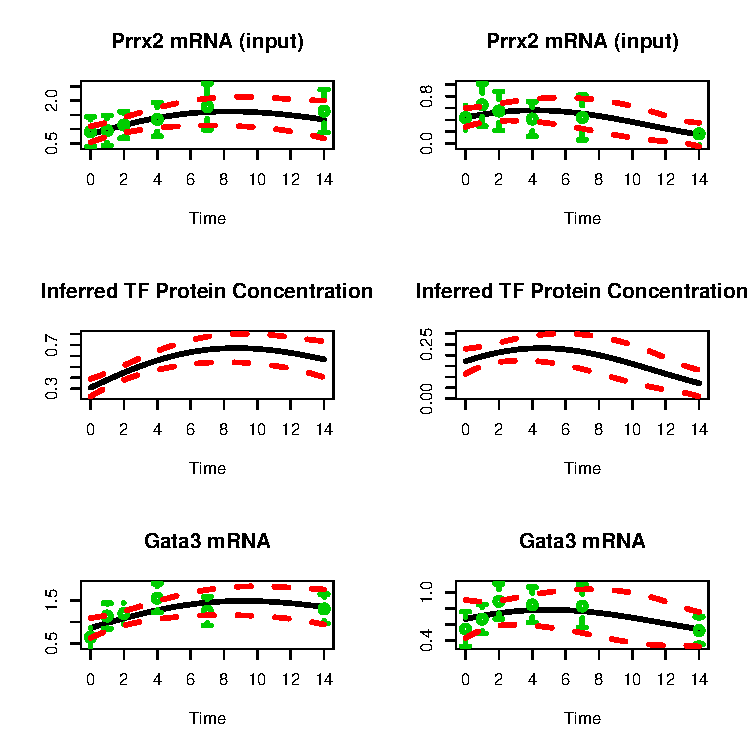
\includegraphics[width=\columnwidth]{gpdisim_Prrx2_Gata3}}
  \subfigure[Tle3 gene: log-likelihood $-0.47$]{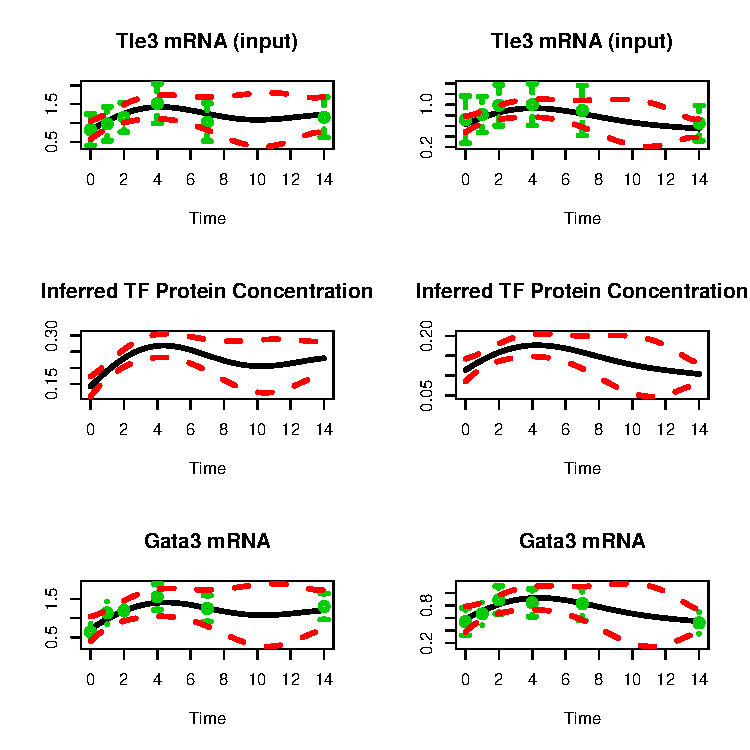
\includegraphics[width=\columnwidth]{gpdisim_Tle3_Gata3}}
  \subfigure[Ctbp2 gene: log-likelihood $-0.67$]{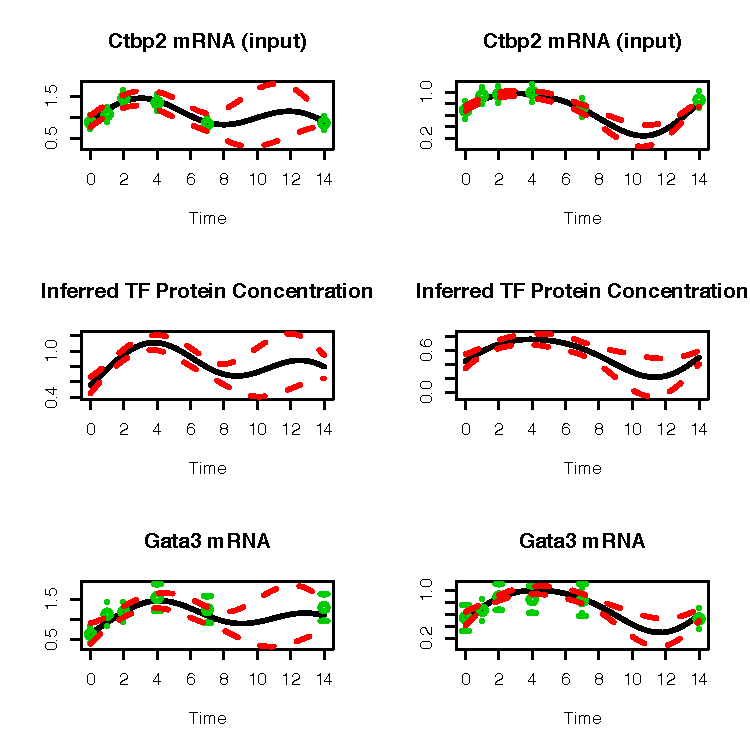
\includegraphics[width=\columnwidth]{gpdisim_Ctbp2_Gata3}}
  \subfigure[Smarcd2 gene: log-likelihood $-1.37$]{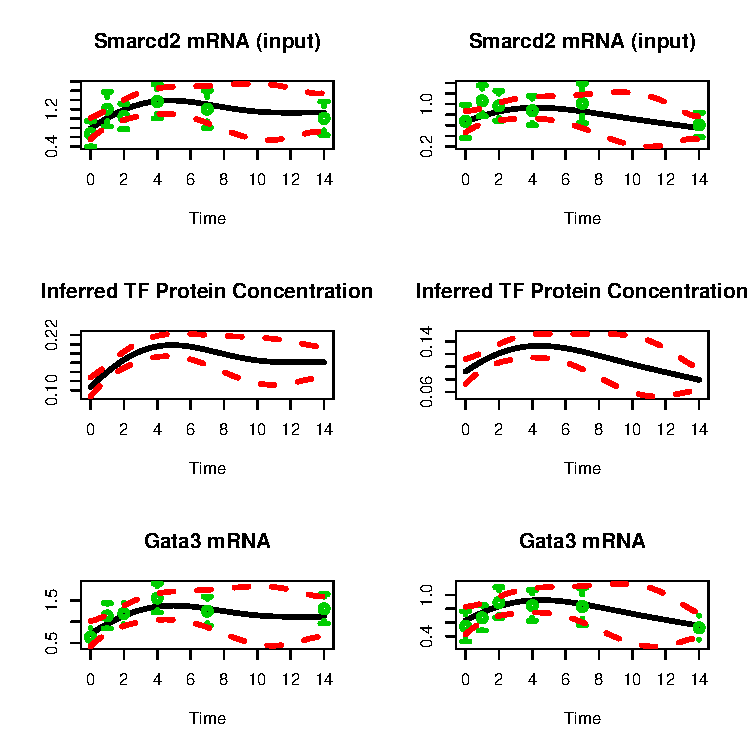
\includegraphics[width=\columnwidth]{gpdisim_Smarcd2_Gata3}}
  \caption{Top-ranking models. In each subplot, the left column shows
    the model for the data from the non-treated experiment and the
    right column for the retinoic acid treated experiment.}
  % \neil{What was the log likelihood? What is on the left and the right? i.e. which is the retanoic acid?}}
  \label{fig:model1}
\end{figure*}

% \begin{figure}[htb]
%   \centering
%   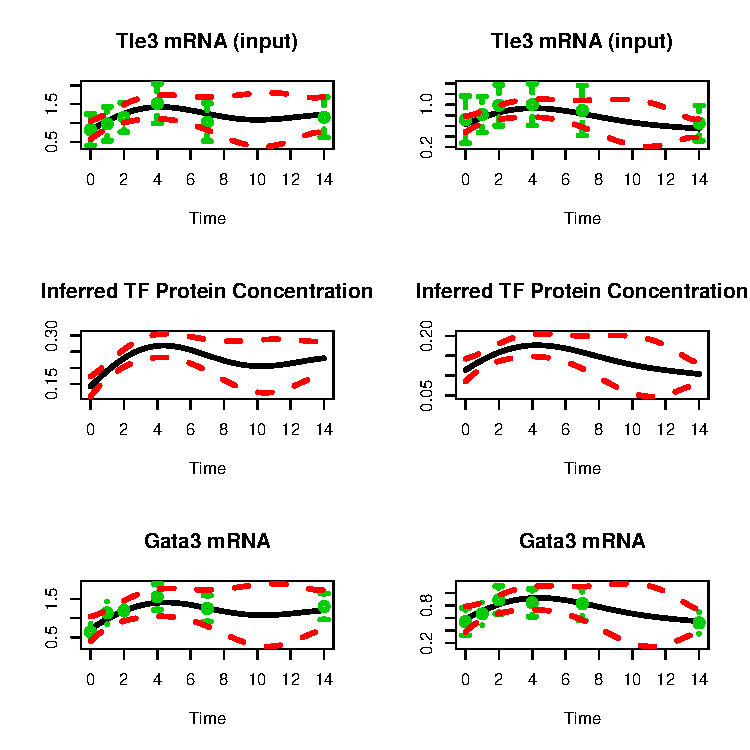
\includegraphics[width=\columnwidth]{gpdisim_Tle3_Gata3}
%   \caption{Top-ranking models}
%   \label{fig:model2}
% \end{figure}

% \begin{figure}[htb]
%   \centering
%   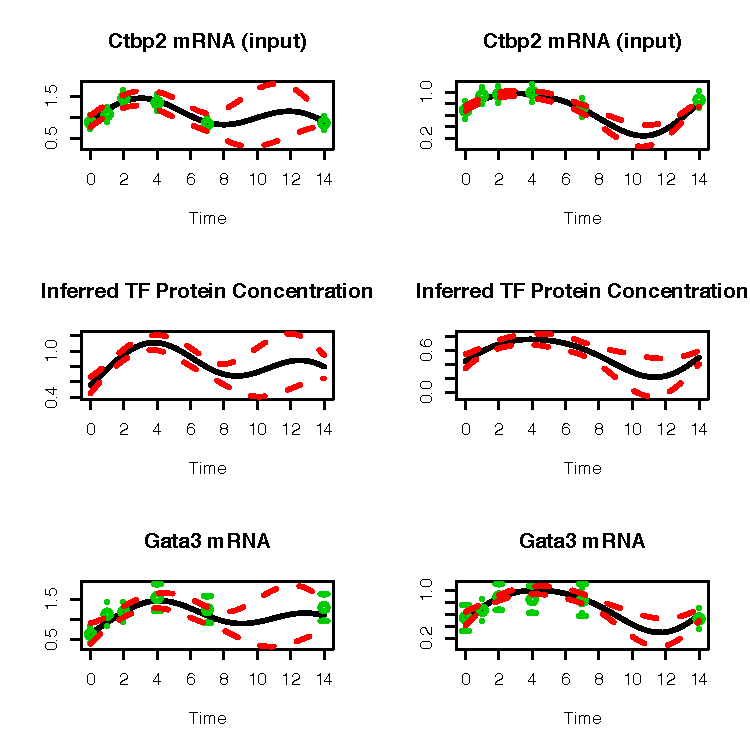
\includegraphics[width=\columnwidth]{gpdisim_Ctbp2_Gata3}
%   \caption{Top-ranking models}
%   \label{fig:model3}
% \end{figure}

% \begin{figure}[htb]
%   \centering
%   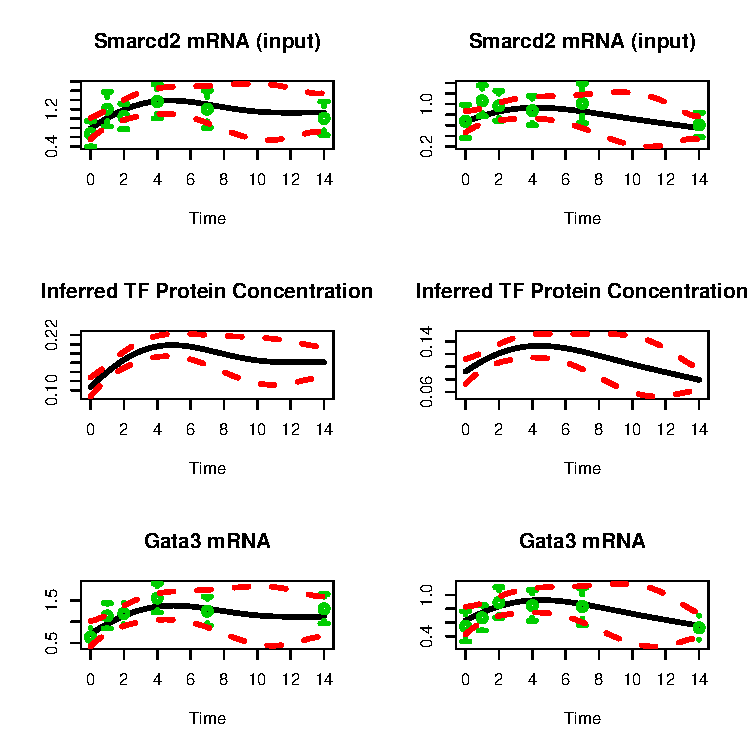
\includegraphics[width=\columnwidth]{gpdisim_Smarcd2_Gata3}
%   \caption{Top-ranking models}
%   \label{fig:model5}
% \end{figure}

\section{Discussion}

While the  presented preliminary results seem  very promising, further
biological verification  is needed to confirm  the predictions.  Given
only the time  series data we have here it  will impossible to predict
with certainty a given relationship. For example the profile that will
emerge if gene A activates  gene B could be indistinguishable from the
profile that arises  if gene B represses gene  A. To disambiguate more
data from  different perturbations  (such as knocking  out one  of the
genes) of  the system  is required. However,  our approach  makes some
preliminary predictions  that could be  used to update  hypotheses and
design  new  experiments.  The  set  of  candidate  regulators is  now
sufficiently  small that  they could  be sifted  using  less expensive
low-throughput techniques.

\small

\bibliographystyle{IEEEabrv}
\bibliography{lawrence,other,zbooks}


\end{document}
